\chapter{非平衡统计力学}

在前面的章节中我们主要研究了各种物理量统计平均值的计算问题,这些平均值以高精度表示出从对 \textcolor{RoyalBlue}{\textbf{\kaishu 处于平衡}} 的给定系统进行有关测量所预期得到的结果。但是,对于近平衡和原理平衡的体系,基于以下几方面的理由,能谱-配分函数-热力学量的研究范式就显得力不从心:

\begin{figure}[ht]
    \centering
    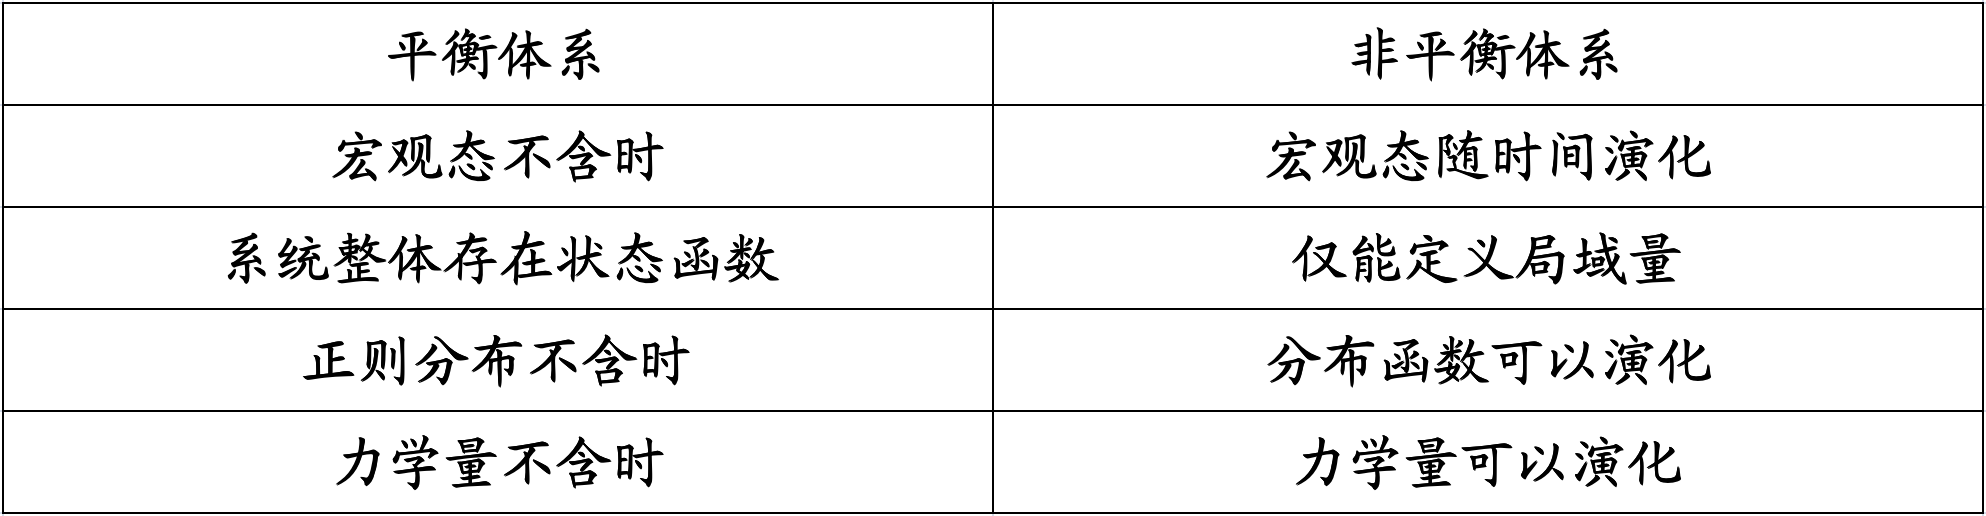
\includegraphics[width=1\textwidth]{figures/equ-nonequ.png}
    \caption{\kaishu 平衡态与非平衡态的区别}
    \label{fig:equ-nonequ}
\end{figure}

由此可见,对于非平衡系统, \textcolor{RoyalBlue}{\textbf{\kaishu 演化}} 二字是核心。本章将从两个方面来研究非平衡系统的演化:一是 \textcolor{RoyalBlue}{\textbf{\kaishu 分布的演化}},即如何从初始分布演化到平衡分布,也就是说一个不处于平衡态的分布函数如何最终逼近平衡分布,并继续维持平衡分布;二是 \textcolor{RoyalBlue}{\textbf{\kaishu 力学量的演化}},即力学量如何从初始状态演化到平衡态,这将涉及关联函数的概念。这两种视角分别相当于量子力学中的薛定谔绘景和海森堡绘景,为了看出这一点,我们必须再次将目光投向 \textcolor{RoyalBlue}{\textbf{\kaishu 刘维尔定理}} 。

\section{再论刘维尔定理}\label{sec:再论刘维尔定理}

对于一个不显含时的力学量 $A$,其演化方程为
\begin{equation}\label{equ:刘维尔定理,不显含时}
    \frac{\mathrm{d} A}{\mathrm{d} t} =  [A, H]
\end{equation}
为了将它写成更一般的微分方程形式,我们定义 \textcolor{RoyalBlue}{\textbf{\kaishu 刘维尔算符}} 为
\begin{equation}\label{equ:刘维尔算符}
    \mathcal{L}A \equiv [A, H]
\end{equation}
这样,\eqref{equ:刘维尔定理,不显含时} 就可以写成
\begin{equation}\label{equ:刘维尔定理,不显含时,微分方程形式}
    \frac{\mathrm{d} A}{\mathrm{d} t} =  \mathcal{L}A
\end{equation}
那么自然而然地,形式解
\begin{equation}\label{equ:形式解}
    A(\Gamma,t) = e^{t\mathcal{L}}A(\Gamma,0)
\end{equation}

代表点密度也是一个特殊的力学量,但由于刘维尔定理的存在,它的演化方程可以写成
\begin{equation}\label{equ:代表点密度的演化方程}
    f(\Gamma,t) =  e^{-t\mathcal{L}}f(\Gamma,0)
\end{equation}

同时,刘维尔算符具有反自伴性(Posson括号的微分性质导致的),即
\begin{align}\label{equ:反自伴性}
    \int (\mathcal{L}A)*B \,\mathrm{d}\Gamma= -\int A*(\mathcal{L}B) \,\mathrm{d}\Gamma \\
    \int (e^{t\mathcal{L}}A)*B \,\mathrm{d}\Gamma= \int A*(e^{-t\mathcal{L}}B) \,\mathrm{d}\Gamma
\end{align}

有了刘维尔算符,我们就可以将力学量的系综平均写为较为简洁的形式。不过这样的平均有两种角度来看待: \textcolor{RoyalBlue}{\textbf{\kaishu 从薛定谔绘景的角度,力学量 $A$ 仅是相点位置的函数 $A(\Gamma)$ ,而占据这些相点的概率分布是随时间变化的}} ,因此力学量的系综平均可以写为
\begin{equation}\label{equ:力学量的系综平均,薛定谔绘景}
    \langle A(t) \rangle = \int A(\Gamma) f(\Gamma, t) \,\mathrm{d}\Gamma
\end{equation}
\textcolor{RoyalBlue}{\textbf{\kaishu 从海森堡绘景的角度,力学量 $A$ 是随时间变化的,而概率分布 $f$ 是相点位置的函数 $f(\Gamma)$ ,不随时间改变}} ,所以力学量的系综平均也可以写为
\begin{equation}\label{equ:力学量的系综平均,海森堡绘景}
    \langle A(t) \rangle = \int A(\Gamma,t) f(\Gamma) \,\mathrm{d}\Gamma
\end{equation}
这二者的联系可以通过如下方式说明:
\begin{align*}
    \int A(\Gamma) f(\Gamma, t) \,\mathrm{d}\Gamma = \int A(\Gamma) e^{-t\mathcal{L}}f(\Gamma,0) \,\mathrm{d}\Gamma \\
    = \int e^{t\mathcal{L}}A(\Gamma) f(\Gamma,0) \,\mathrm{d}\Gamma = \int A(\Gamma,t) f(\Gamma) \,\mathrm{d}\Gamma
\end{align*}
\begin{justification}{\kaishu 反思与质疑}
\kaishu \fontsize{11pt}{16pt}
    这里直接将依赖关系隐去可能会导致一定程度的困惑,但是必须牢记,我们观察对 $A(t)$ 所有实验可能值的平均值时, \textcolor{RoyalBlue}{\textbf{\kaishu  所抽取的样本来自初始条件的分布}},也就是说
    \[
        \langle A(t) \rangle = \int A(\Gamma_0\rightarrow \Gamma_t) f(\Gamma_0; \text{time} = 0) \,\mathrm{d}\Gamma_0 = \int A(\Gamma_0;\text{time} = 0) f(\Gamma_0,t) \,\mathrm{d}\Gamma_0
    \]
    前者是海森堡绘景,后者是薛定谔绘景,被积变量总是遍历整个相空间,所以 $\mathrm{d}\Gamma_0 = \mathrm{d}\Gamma$ 。
\end{justification}

此外,平衡分布是一个与系统哈密顿量对易的力学量:
\begin{equation}\label{equ:平衡分布和哈密顿量对易}
    f_{eq}(H) = \frac{e^{-\beta H}}{Z} ,\quad\mathcal{L}f_{eq}(H) = [f_{eq}(H), H] = 0
\end{equation}

所以,与平衡系统不同,对于非平衡系统我们有两种方式来求一个力学量的系综平均,即 \eqref{equ:力学量的系综平均,薛定谔绘景} 和 \eqref{equ:力学量的系综平均,海森堡绘景} 。运用前者,我们将从 \textcolor{RoyalBlue}{\textbf{\kaishu 布朗运动}} 开始,研究分布函数随时间的演化,导出其所满足的偏微分方程,即 \textcolor{RoyalBlue}{\textbf{\kaishu 福克尔-普朗克方程}} ;运用后者,我们将力学量视为随机过程,引入 \textcolor{RoyalBlue}{\textbf{\kaishu 关联函数}} ,建立其与 \textcolor{RoyalBlue}{\textbf{\kaishu 响应函数}} 的联系,研究 \textcolor{RoyalBlue}{\textbf{\kaishu 涨落耗散定理}} 。

\section{分布的演化:薛定谔绘景}\label{sec:分布的演化:薛定谔绘景}

\subsection{布朗运动的爱因斯坦理论}

在薛定谔绘景下,我们希望研究系统分布的演化,其中最常见的就是坐标分布的演化,也就是 \textcolor{RoyalBlue}{\textbf{\kaishu 扩散行为}}。而粒子扩散的根源在于周围的液体分子对布朗粒子进行的永不停歇的和不同程度上是随机的撞击。这样一来,如果追踪单一布朗粒子的运动,我们发现它可以被看做一种步长为 $l$ 、频率为 $\tau$ 的 \textcolor{RoyalBlue}{\textbf{\kaishu 随机行走问题}} ,其中 $l$ 为粒子平均自由程,$\tau$ 为粒子平均自由时间。同时,粒子所行走的每一步都是独立同分布的:
\begin{equation}\label{equ:S_N}
    S_N = \sum_{i=1}^N X_i,\quad X_i = \left\{\begin{array}{lll}
        ~~~1 & P = 0.5 \\
        -1& P = 0.5
        \end{array}\right.
\end{equation}
其中 $X_i$ 独立同分布。根据中心极限定理,当 $N\rightarrow \infty$ 时,$S_N$ 的分布趋于正态分布,即
\begin{equation}\label{equ:S_N的分布}
    P(S_N = n)\mathrm{d}n = \frac{1}{\sqrt{2\pi N}}\exp\left(-\frac{n^2}{2N}\right) \mathrm{d}n
\end{equation}
粒子平均 $\tau$  时间做一次随机跳跃,所以 $N = t / \tau$ ,同时做变量代换 $x = nl$ ,则粒子在 $N$ 步后的位置 $x$ 的概率分布为
\begin{equation}\label{equ:布朗运动的概率分布}
    P(x,t)\mathrm{d}x = P(S_N = n)\mathrm{d}n = \frac{1}{\sqrt{2\pi t / \tau}}\exp\left(-\frac{x^2}{2t / \tau}\right) \mathrm{d}x
\end{equation}
令 $D = \frac{1}{2} l^2/\tau$ ,我们就可以得到非常标准的扩散方程的一个解:
\begin{equation}\label{equ:扩散方程的解}
    P(x,t) = \frac{1}{\sqrt{4\pi Dt}}\exp\left(-\frac{x^2}{4Dt}\right)
\end{equation}
这里引入的 $D$ 与给定系统的宏观 \textcolor{RoyalBlue}{\textbf{\kaishu 扩散系数}} 完全相同,也就是说微观量 $l,\tau$ 和宏观量 $D$ 建立起了联系。三维情况下,由于各维度独立,所以联合概率密度等于边缘概率密度的乘积:
\begin{equation}\label{equ:三维扩散方程}
    P(\bm{r},t) = \frac{1}{(4\pi Dt)^{3/2}}\exp\left(-\frac{\bm{r}^2}{4Dt}\right)
\end{equation}
\begin{justification}{反思与质疑}
\kaishu \fontsize{11pt}{16pt}
    \quad\quad  三维扩散方程的形式为
    \[
        \frac{\partial }{\partial t}n(\bm r, t) = D\nabla^2 n(\bm r, t)
    \]
    通过傅里叶变换,方程的解正好就是 \eqref{equ:三维扩散方程} 的解,其中的道理蕴含在概率与统计的关系中:扩散方程作为唯像的总结,它所描述的结果是统计性的,而这样的统计性是对单一粒子大量抽样的结果,而在大数定律的极限下将会收敛于概率本身。因此,扩散方程的解正好就是随机过程的解,而随机过程的解也正好就是扩散方程的解。
\end{justification}

那么这样一来,借助分布函数 \eqref{equ:三维扩散方程} 式,我们可以求得布朗粒子的方均位移为
\begin{equation}\label{equ:布朗粒子的方均位移}
    \langle r^2(t) \rangle = \int_{-\infty}^{+\infty} \bm r^2 P(x,t)\mathrm{d}x = 6Dt
\end{equation}

可以看到,最初集聚在原点的布朗粒子系综随着时间的增加而扩散出去,并且这种行为宏观上显然是不可逆的,并且无论我们把注意力放在单一粒子上,还是放在粒子系综上,都可以看到这种不可逆性。这个现象的最终根源在于布朗粒子受到流体中分子永不停息、或多或少是随机的碰撞。换句话说,\textcolor{RoyalBlue}{\textbf{\kaishu  这个现象的不可逆性归根结底来源于流体分子对布朗粒子所施加的随机力的涨落}} 。

\subsection{福克尔-普朗克方程}

抄 pathria

\section{力学量的演化:海森堡绘景}\label{sec:力学量的演化:海森堡绘景}


\subsection{关联函数及其稳态性质}

抄笔记

\subsection{布朗运动的朗之万理论}

在布朗运动的爱因斯坦理论中我们已经指出,布朗粒子的不可逆运动来自流体分子所施加随机力的涨落,现在我们来看看这种涨落的统计性质。首先,我们来考虑一个布朗粒子在 $t$ 时刻的速度 $v(t)$ ,它是由于流体分子的碰撞而产生的随机力 $f(t)$ 所引起的,而这个随机力 $f(t)$ 的统计性质是已知的,即
\begin{equation}\label{equ:随机力的统计性质}
    \langle f(t) \rangle = 0, \quad \langle f(t)f(t') \rangle = 2m\gamma k_BT\delta(t-t')
\end{equation}


<-- 抄pathria,给出唯像的朗之万方程、爱因斯坦关系,并指出爱因斯坦关系是涨落耗散定理的一种表述形式 -->

\section{线性响应与涨落耗散定理}\label{sec:线性响应与涨落耗散定理}

\subsection{昂萨格回归假说}

首先从回归假说的神秘性开始,即自然涨落和弛豫不可分辨,抄一点chandler,指出在扩散中的应用。

\subsection{静态响应与静态弛豫}

研究静态弛豫,证明假说的正确性,抄笔记

\subsection{响应函数}

一般情况的弛豫——定义响应函数,物理意义、因果性、稳态性,抄笔记

指出响应函数与关联函数的关系,这就是涨落耗散定理

\subsection{从线性响应理论到朗之万方程}

三个关键认识

\section{总结}\label{sec:非平衡总结}
